\documentclass[9pt, aspectratio=169, xcolor=table]{beamer}

\usetheme{UR}
\usepackage{pgf}
\usepackage{tcolorbox}
\usepackage{tikz, calc}
\usepackage{hyperref}
\usetikzlibrary{shapes,arrows,positioning,calc}
\usetikzlibrary{arrows,automata}
\tikzstyle{state}=[circle, fill=red,draw=none,text=white, minimum size =0.8cm]
\tikzstyle{graph node}=[circle, fill=blue,draw=none,text=white, minimum size =0.8cm]
\usepackage{epsfig, amsfonts, amsbsy, amsmath,pifont,amssymb}
\usetikzlibrary{shapes,arrows,automata}
\usepackage[ruled,vlined]{algorithm2e}
\usepackage{hyphenat}
\usepackage{booktabs}
\usepackage{multirow}
\usepackage{tcolorbox}
\input{./style_files_ur/mysymbol.sty}
\input{./style_files_ur/my_beamer_defs.sty}
\input{./figures/tikz_styles}

\newcommand{\EE}{{\mathbb E}}
\newcommand{\bbeps}{{\boldsymbol{\epsilon}}}
\newcommand{\clip}{\boldsymbol{\phi}}
\newcommand{\bo}{\mathbf{o}}
\newcommand{\mymod}{\mathrm{mod}_N}
\newcommand{\QED}{\hfill\ensuremath{\blacksquare}}
\newcommand{\cmark}{\ding{51}}%
\newcommand{\xmark}{\ding{55}}%

\DeclareMathOperator{\Tr}{Trace}
\DeclareMathOperator{\vvec}{vec}

\logo{
\includegraphics[width=0.32in]{./style_files_ur/ur_logo.png}}

\newtcolorbox{myblockt}[1]{colback=urblue!5!white,
	colframe=urblue,fonttitle=\bfseries,
	title=#1}

\newtcolorbox{myblock}{colback=urblue!5!white,
	colframe=urblue,fonttitle=\bfseries}

%%%%%   University of Rochester yellow + blue theme accents   %%%%%
%  Dandelion-yellow lettering on the deep-blue banners (title page,
%  frame-title bars), with blue structural elements (bullets, rules).
\setbeamercolor{frametitle}{fg=white,bg=urblue}
\setbeamercolor{title}{fg=white,bg=urblue}
\setbeamercolor{titlelike}{fg=white,bg=urblue}
\setbeamercolor{structure}{fg=urblue}
\setbeamercolor{item}{fg=urblue}
\setbeamercolor{section in toc}{fg=urblue}
% turn the red navigation strip / footer into UR yellow (blue lettering)
\setbeamercolor{palette quaternary}{fg=urblue,bg=uryellow}
\setbeamercolor{section in head/foot}{fg=urblue,bg=uryellow}
\setbeamercolor{subsection in head/foot}{fg=urblue,bg=uryellow}
\setbeamercolor{author in head/foot}{fg=urblue,bg=uryellow}
\setbeamercolor{title in head/foot}{fg=urblue,bg=uryellow}

\begin{document}

\author[\urblue{Online DAG Learning from Streaming Data}]{\begin{tabular}{c}
		{\large Hamed Ajorlou}\svpos  \\
		{\small Dept. of ECE and Goergen Institute for Data Science and AI} \\
		{\small University of Rochester}  \\
		{\small \href{mailto:hajorlou@ur.rochester.edu}{hajorlou@ur.rochester.edu}} \\
		\\
		{\small \urblue{\textbf{Collaborators:}} Gonzalo Mateos and Mariano Tepper}
		\\
		{\small \urblue{\textbf{Acknowledgment:}} NSF Award ECCS-2231036}
\end{tabular}}


\date[2026]{2026}
\title[\urblue{DyCoLiDE}]{{\Large Online DAG Learning\\from Streaming Observational Data}}
\institute[Dept. of ECE~~--~~University of Rochester]{}

\frame{\titlepage}

%%%%%%%%%%%%%%%%%%%%%%%%%%%%%%%%%%%%%%%%%%%%%%%%%%%%%%%%%%%%%%%%%%%%%%%%%%%%%%%%
%%%   S   L   I   D   E   %%%%%%%%%%%%%%%%%%%%%%%%%%%%%%%%%%%%%%%%%%%%%%%%%%%%%%
%%%%%%%%%%%%%%%%%%%%%%%%%%%%%%%%%%%%%%%%%%%%%%%%%%%%%%%%%%%%%%%%%%%%%%%%%%%%%%%%
\frame{\frametitle{Learning from relational data}

	\bi  \blue{Graphs are natural models for relational data} that help us \green{learn} in timely \red{applications}	\ei

	\bfig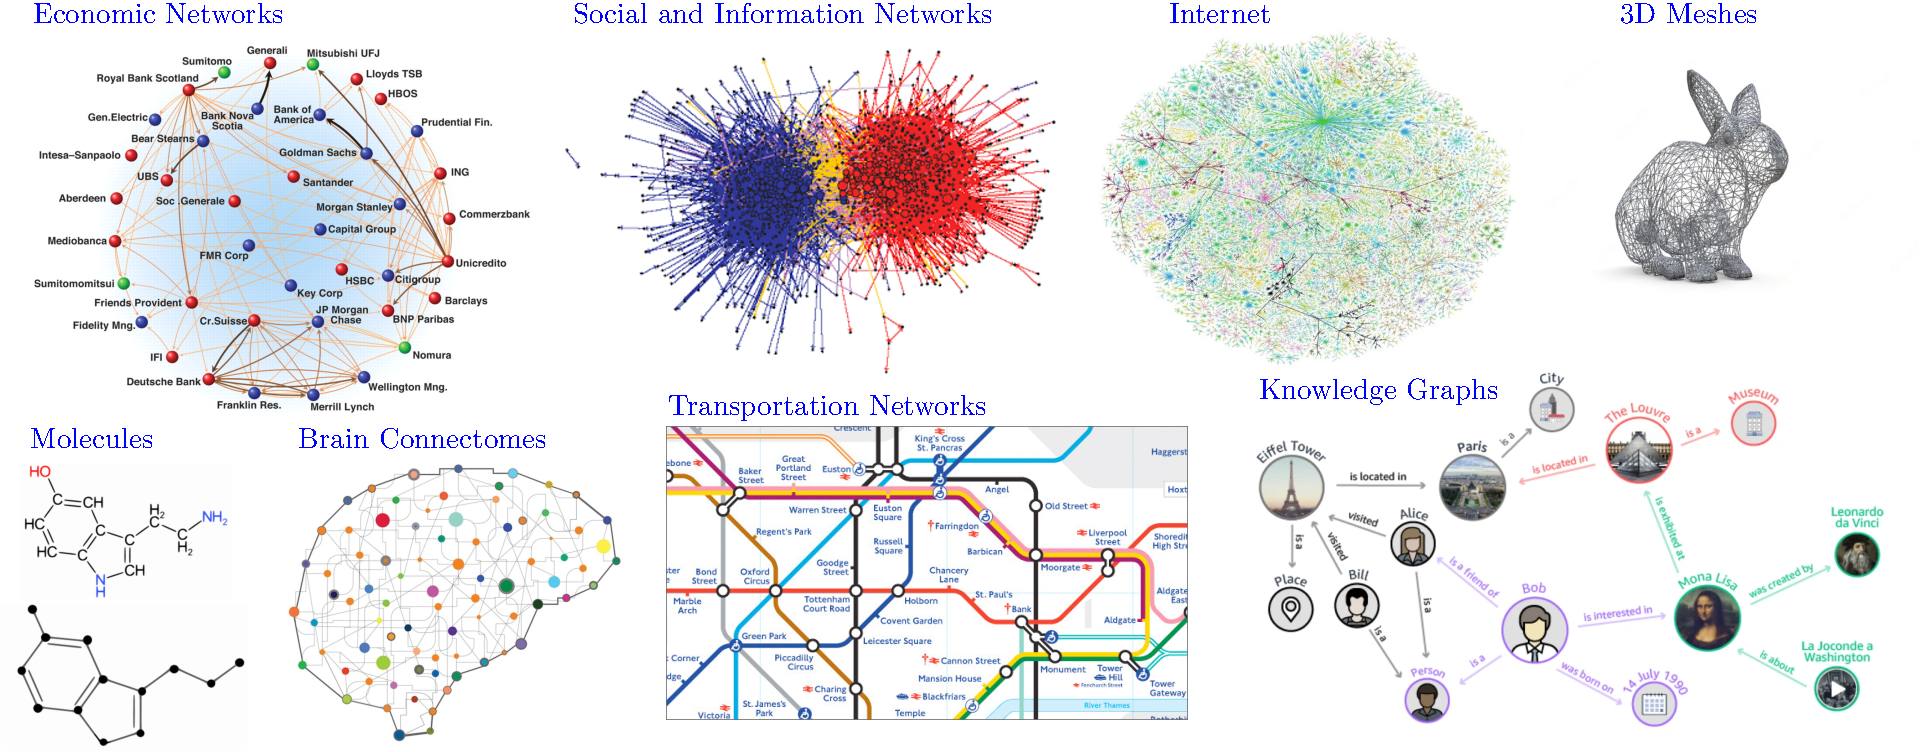
\includegraphics[scale=0.45]{figures/graphs_everywhere.pdf}\efig

}

%%%%%%%%%%%%%%%%%%%%%%%%%%%%%%%%%%%%%%%%%%%%%%%%%%%%%%%%%%%%%%%%%%%%%%%%%%%%%%%%
%%%   S   L   I   D   E   %%%%%%%%%%%%%%%%%%%%%%%%%%%%%%%%%%%%%%%%%%%%%%%%%%%%%%
%%%%%%%%%%%%%%%%%%%%%%%%%%%%%%%%%%%%%%%%%%%%%%%%%%%%%%%%%%%%%%%%%%%%%%%%%%%%%%%%
\frame{\frametitle{Learning the structure of directed acyclic graphs}\svpos

	\bc
	\col{0.78}
	\bi \red{\textbf{Goal:}} learn the structure of \blue{directed acyclic graphs (DAGs)} from observational data
	\ei

	\bi DAGs are prominent models across ML and the sciences
	\ai Conditional independences among variables in Bayesian networks
	\ai DAG edges may carry \green{causal interpretations}
	\ai Bio \darkgray{\small [Sachs et al'05]}, finance \darkgray{\small [Sanford-Moosa'12]}, healthcare \darkgray{\small [Lucas'04]}
	\ei

	\bi \textbf{Challenges:} directionality, acyclicity (combinatorial constraint), identifiability, NP-hard search \darkgray{\small [Chickering'96]}\ei
	\col{0.20}
	\def \myfactor{0.7}
{\fontsize{8}{8}\selectfont
\begin{tikzpicture}[auto, node distance=1.25cm, every loop/.style={},
                    thick,main node/.style={circle,draw}, scale = \myfactor]
\tikzstyle{stuff_fill}=[node,draw,fill=black!20]

\node[main node] (1) [draw=urblue!80,fill=uryellow!30] {1};
\node[main node] (2) [below left of=1] [draw=urblue!80,fill=uryellow!30] {2};
\node[main node] (3) [below right of=1] [draw=urblue!80,fill=uryellow!30] {3};
\node[main node] (4) [below right of=2] [draw=urblue!80,fill=uryellow!30] {4};
\node[main node] (5) [below of=4] [draw=urblue!80,fill=uryellow!30] {5};

\draw [->, color=urblue] (1) -- (2);
\draw [->, color=urblue] (1) -- (3);
\draw [->, color=urblue] (1) -- (4);
\draw [->, color=urblue] (1) to [out=30,in=90] ($(3.east)+(0.5cm, -0.5cm)$) to [out=-90,in=0] (5);
\draw [->, color=urblue] (2) -- (4);
\draw [->, color=urblue] (3) -- (4);
\draw [->, color=urblue] (4) -- (5);
\draw [->, color=urblue] (3) to [out=-90,in=45]  (5);

% \draw [dashed, ->, color=darkred] (5) to [out=180,in=-90]  ($(2.west)+(-0.5cm,-0.5cm)$)
                                    % to [out=90,in=150] (1);

\end{tikzpicture}}
	\ec

	\pause

	\begin{myblock}
		\bi \red{\textbf{This work:}} 
        presents a DAG-learning framework that is capable of mini-batch data processing on causal data, which makes it possible to dynamically infer connectivity of causal networks
        
        
        \ei
	\end{myblock}

}
%%%%%%%%%%%%%%%%%%%%%%%%%%%%%%%%%%%%%%%%%%%%%%%%%%%%%%%%%%%%%%%%%%%%%%%%%%%%%%%%
%%%   S   E   C   T   I   O   N   %%%%%%%%%%%%%%%%%%%%%%%%%%%%%%%%%%%%%%%%%%%%%%
%%%%%%%%%%%%%%%%%%%%%%%%%%%%%%%%%%%%%%%%%%%%%%%%%%%%%%%%%%%%%%%%%%%%%%%%%%%%%%%%
\section{Background: Linear causal models and DAG learning}
\begin{frame} \frametitle{Roadmap} \tableofcontents \end{frame}

%%%%%%%%%%%%%%%%%%%%%%%%%%%%%%%%%%%%%%%%%%%%%%%%%%%%%%%%%%%%%%%%
%%%   S   L   I   D   E   %%%%%%%%%%%%%%%%%%%%%%%%%%%%%%%%%%%%%%
%%%%%%%%%%%%%%%%%%%%%%%%%%%%%%%%%%%%%%%%%%%%%%%%%%%%%%%%%%%%%%%%

\begin{frame}[shrink=20]{Linear structural (causal) models}

	\begin{minipage}[t]{0.82\textwidth}
		\bi DAG $\ccalG(\ccalV,\ccalE)$, vertices $\ccalV=\{1,\ldots,d\}$, weighted \darkgreen{adjacency} $\darkgreen{\bbW}\in\reals^{d\times d}$
		\ai $W_{ij}\neq 0$ encodes a directed causal link $i\to j$ \ei

		\bi \blue{Linear structural equation model (SEM):} each node a noisy linear combination of its parents
		\be \red{\bbX} = \red{\bbX}\darkgreen{\bbW} + \bbZ \ee
		\ai Rows of $\bbX\in\reals^{n\times d}$ are i.i.d. samples; $\bbZ$ collects exogenous noise
		\ai \orange{Equal variance (EV):} $Z_{ij}\sim\ccalN(0,\sigma^2)$ \quad
		\orange{Non-equal (NV):} $Z_{ij}\sim\ccalN(0,\sigma_j^2)$ \ei \svpos

		\pause

		\bi \blue{Structural vector autoregressive (SVAR):} adds $p$ lagged terms
		\be \bbx_t = \darkgreen{\bbW}^\top\bbx_t + \sum_{k=1}^{p}\darkpurple{\bbA_k}^\top\bbx_{t-k} + \bbz_t
		\quad\Longrightarrow\quad \red{\bbX}=\red{\bbX}\darkgreen{\bbW}+\bbY\darkpurple{\bbA}+\bbZ \ee
		\ai $\bbY=[\bbX_{-1},\ldots,\bbX_{-p}]$ stacks lags; $\darkpurple{\bbA}\in\reals^{pd\times d}$ stacks $\{\bbA_k\}$
		\ai Acyclicity constrains \darkgreen{$\bbW$} only -- temporal order rules out cycles in \darkpurple{$\bbA$}\ei
	\end{minipage}
	%
	\begin{minipage}[t]{0.12\textwidth}
		\vpos \svpos
		\bfig
		\centering
		\def \myfactor{0.7}
{\fontsize{8}{8}\selectfont
\begin{tikzpicture}[auto, node distance=1.25cm, every loop/.style={},
                    thick,main node/.style={circle,draw}, scale = \myfactor]
\tikzstyle{stuff_fill}=[node,draw,fill=black!20]

\node[main node] (1) [label=above:\darkred{$\bbx_{1}$},draw=urblue!80,fill=uryellow!30] {1};
\node[main node] (2) [below left of=1] [label=left:\darkred{$\bbx_{2}$},draw=urblue!80,fill=uryellow!30] {2};
\node[main node] (3) [below right of=1] [label=right:\darkred{$\bbx_{3}$},draw=urblue!80,fill=uryellow!30] {3};
\node[main node] (4) [below right of=2] [label=left:\darkred{$\bbx_{4}$},draw=urblue!80,fill=uryellow!30] {4};
\node[main node] (5) [below of=4] [label=below:\darkred{$\bbx_{5}$},draw=urblue!80,fill=uryellow!30] {5};

\draw [->, color=urblue] (1) -- node [swap] {\darkgreen{$W_{12}$}} (2);
\draw [->, color=urblue] (1) -- node {\darkgreen{$W_{13}$}} (3);
\draw [->, color=urblue] (1) -- node {\darkgreen{$W_{14}$}} (4);
\draw [->, color=urblue] (1) to [out=30,in=90] ($(3.east)+(1.25cm, -0.5cm)$) to [out=-90,in=-15] node {\darkgreen{$W_{15}$}}(5);
\draw [->, color=urblue] (2) -- node [swap] {\darkgreen{$W_{24}$}} (4);
\draw [->, color=urblue] (3) -- node {\darkgreen{$W_{34}$}} (4);
\draw [->, color=urblue] (4) -- node [swap] {\darkgreen{$W_{45}$}} (5);
\draw [->, color=urblue] (3) to [out=-70,in=30] node {\darkgreen{$W_{35}$}} (5);

% \draw [dashed, ->, color=darkred] (5) to [out=180,in=-90]  ($(2.west)+(-0.5cm,-0.5cm)$)
                                    % to [out=90,in=150] (1);

\end{tikzpicture}}
		\efig
	\end{minipage}

	\pause
	\begin{myblock}
	\bi \darkpurple{\textbf{Q:}} estimate \darkgreen{$\bbW$} (and \darkpurple{$\bbA$}) from data revealed \red{sequentially over time}?\ei
	\end{myblock}
\end{frame}

%%%%%%%%%%%%%%%%%%%%%%%%%%%%%%%%%%%%%%%%%%%%%%%%%%%%%%%%%%%%%%%%
%%%   S   L   I   D   E   %%%%%%%%%%%%%%%%%%%%%%%%%%%%%%%%%%%%%%
%%%%%%%%%%%%%%%%%%%%%%%%%%%%%%%%%%%%%%%%%%%%%%%%%%%%%%%%%%%%%%%%

\begin{frame}{Stability of the SVAR model}\svpos

	\bi The SVAR is only a \blue{valid generative model} if the underlying process is \green{stationary} -- otherwise $\bbx_t$ \red{diverges} \darkgray{\small [L\"utkepohl'05]} \ei \svpos

	\bi Solve the contemporaneous part to get the \darkpurple{reduced-form VAR}:
	\be \bbx_t = \darkgreen{\bbW}^\top\bbx_t + \sum_{k=1}^{p}\darkpurple{\bbA_k}^\top\bbx_{t-k} + \bbz_t \;\;\Longrightarrow\;\; \bbx_t=\sum_{k=1}^{p}\bbC_k^\top\bbx_{t-k}+(\bbI_d-\darkgreen{\bbW})^{-\top}\bbz_t \ee
	\ai \blue{Evolution operator} $\bbC_k=(\bbI_d-\darkgreen{\bbW})^{-\top}\darkpurple{\bbA_k}^\top$ -- the lag matrices act \red{through} the inverted instantaneous structure \ei \svpos

	\bi Stack the $p$ lags into the $pd\times pd$ \orange{companion matrix} $\bbF$ \darkgray{\small [Hamilton'94]}:
	\be \bbF=\begin{bmatrix} \bbC_1^\top & \bbC_2^\top & \cdots & \bbC_p^\top \\ \bbI_d & & & \\ & \ddots & & \\ & & \bbI_d & \end{bmatrix},
	\qquad \darkpurple{\textbf{Stability}}\;\Longleftrightarrow\; \rho(\bbF)=\max_i|\lambda_i(\bbF)|<1 \ee
	\ai In our data generator we enforce a \green{safety margin} $\rho(\bbF)<0.95$\ei \svpos

	\pause

	\begin{myblock}
		\bi \red{\textbf{Why we care:}} stability $\Rightarrow$ \blue{stationarity} $\Rightarrow$ the second-order statistics $(\bbSigma_{XX},\bbSigma_{XY},\bbSigma_{YY})$ \green{exist and are finite} -- precisely the limits our running estimates track\ei
	\end{myblock}

\end{frame}

%%%%%%%%%%%%%%%%%%%%%%%%%%%%%%%%%%%%%%%%%%%%%%%%%%%%%%%%%%%%%%%%
%%%   S   L   I   D   E   %%%%%%%%%%%%%%%%%%%%%%%%%%%%%%%%%%%%%%
%%%%%%%%%%%%%%%%%%%%%%%%%%%%%%%%%%%%%%%%%%%%%%%%%%%%%%%%%%%%%%%%

\begin{frame}{Stability: consequences for learning}\svpos

	\bi \blue{\textbf{(1) Batch-consistency hinges on it.}} Our \darkpurple{streaming} guarantee is $\bbSigma_{\cdot,t}\!\to\!\bbSigma_\cdot$ as $t\!\to\!\infty$ \svpos
	\ai A stationary limit \red{exists only if} $\rho(\bbF)<1$ \darkgray{\small [L\"utkepohl'05]} -- when unstable, $\bbx_t$ diverges and the \orange{running covariance never settles}, so ``covariance is all you need'' breaks down\ei \svpos

	\bi \blue{\textbf{(2) A recovery--stability tension.}} The margin $\rho(\bbF)<1$ \orange{caps the magnitude} of the temporal coefficients $\darkpurple{\bbA}$ \svpos
	\ai Near the stability boundary, true temporal edges stay \red{weak} -- many fall below the detection threshold
	\ai Explains why \darkpurple{$\bbA$}-SHD is \darkred{harder and floors} while \darkgreen{$\bbW$} is recovered near-exactly \darkgray{\small [cf.\ DyCoLiDE results]}\ei \svpos

	\pause

	\begin{myblock}
		\bi \green{\textbf{(3) Guaranteeing stable ground truth.}} We draw stable systems by \blue{rejection sampling} \darkgray{\small [DYNOTEARS, Pamfil et al'20]}: redraw $(\darkgreen{\bbW},\darkpurple{\bbA})$ and \orange{decay the temporal strength $\times0.8$} per attempt until $\rho(\bbF)<0.95$\ei
	\end{myblock}

\end{frame}

%%%%%%%%%%%%%%%%%%%%%%%%%%%%%%%%%%%%%%%%%%%%%%%%%%%%%%%%%%%%%%%%
%%%   S   L   I   D   E   %%%%%%%%%%%%%%%%%%%%%%%%%%%%%%%%%%%%%%
%%%%%%%%%%%%%%%%%%%%%%%%%%%%%%%%%%%%%%%%%%%%%%%%%%%%%%%%%%%%%%%%

\begin{frame}{Continuous optimization for DAG learning}\svpos

	\bi Recovering \darkgreen{$\bbW$} from data is \darkred{NP-hard} as a search over DAGs \darkgray{\small [Chickering'96]} \svpos
	\ai \blue{Key idea} \darkgray{\small [NOTEARS, Zheng et al'18]}: replace the combinatorial constraint with a \orange{smooth acyclicity function} $h(\bbW)=0 \iff \bbW$ acyclic \ei \svpos

	\be \min_{\bbW\in\reals^{d\times d}} \;\ell(\bbW;\bbX) + \lambda\|\bbW\|_1 \quad \mathrm{s.t.}\quad h(\bbW)=0 \ee \svpos

	\bi \darkpurple{Acyclicity functions:}
	\ai NOTEARS: $h_{\mathrm{NT}}(\bbW)=\Tr(e^{\bbW\odot\bbW})-d$
	\ai \red{DAGMA} \darkgray{\small [Bello et al'22]}: $h_s(\bbW)=-\log\det(s\bbI_d-\bbW\odot\bbW)+d\log s$ -- better gradients\ei \svpos

	\pause

	\bi \green{\textbf{CoLiDE}} \darkgray{\small [Saboksayr et al'24]}: jointly estimate the \orange{noise scale} $\sigma$ with $\bbW$
	\begin{myblock}
		\be S(\darkgreen{\bbW},\orange{\sigma};\bbX) = \frac{1}{2n\orange{\sigma}}\|\bbX-\bbX\darkgreen{\bbW}\|_F^2 + \frac{d\orange{\sigma}}{2} + \lambda\|\darkgreen{\bbW}\|_1 \ee
	\end{myblock}
	\ai Decouples $\lambda$ from $\sigma$; closed-form $\sigma$ update; handles heteroscedastic noise (NV)\ei

\end{frame}

%%%%%%%%%%%%%%%%%%%%%%%%%%%%%%%%%%%%%%%%%%%%%%%%%%%%%%%%%%%%%%%%
%%%   S   L   I   D   E   %%%%%%%%%%%%%%%%%%%%%%%%%%%%%%%%%%%%%%
%%%%%%%%%%%%%%%%%%%%%%%%%%%%%%%%%%%%%%%%%%%%%%%%%%%%%%%%%%%%%%%%

\begin{frame}{The gap: batch vs.\ streaming}\svpos

	\bi NOTEARS, GOLEM, DAGMA, CoLiDE, Dynotears, PCMCI \ldots\ all assume the \red{full dataset is available a priori} and revisited every iteration \ei \svpos

	\bi But many modern processes generate data \blue{sequentially}: financial markets, sensor networks, industrial monitoring, biological dynamics \darkgray{\small [time series]} \ei \svpos

	\bi \orange{Retraining from scratch} on each new sample is computationally wasteful -- and the underlying graph may \darkred{drift over time}\ei \svpos

	\pause

	\begin{myblock}
		\bi \red{\textbf{This work -- an online DAG learner that:}}
		\ai processes observations in \blue{mini-batches}, including the true-online $\mathrm{batch\_size}=1$ regime
		\ai handles \green{both SEM and SVAR} generative models
		\ai keeps per-step cost \orange{independent of} the cumulative sample count
		\ai \darkpurple{tracks} time-varying DAGs through abrupt structural change\ei
	\end{myblock}

\end{frame}

%%%%%%%%%%%%%%%%%%%%%%%%%%%%%%%%%%%%%%%%%%%%%%%%%%%%%%%%%%%%%%%%
%%%   S   E   C   T   I   O   N   %%%%%%%%%%%%%%%%%%%%%%%%%%%%%%
%%%%%%%%%%%%%%%%%%%%%%%%%%%%%%%%%%%%%%%%%%%%%%%%%%%%%%%%%%%%%%%%
\section{Online problem formulation}
\begin{frame} \frametitle{Roadmap} \tableofcontents[currentsection] \end{frame}

%%%%%%%%%%%%%%%%%%%%%%%%%%%%%%%%%%%%%%%%%%%%%%%%%%%%%%%%%%%%%%%%
%%%   S   L   I   D   E   %%%%%%%%%%%%%%%%%%%%%%%%%%%%%%%%%%%%%%
%%%%%%%%%%%%%%%%%%%%%%%%%%%%%%%%%%%%%%%%%%%%%%%%%%%%%%%%%%%%%%%%

\begin{frame}{Streaming data model}\svpos

	\bi Sequential protocol indexed by $t=1,2,\ldots$; at time $t$ the learner receives a batch
	\be \bbX_t\in\reals^{n_t\times d}, \qquad N_t=\sum_{\tau=1}^{t}n_\tau \;\;\text{(cumulative size)} \ee
	\ai \blue{$n_t=1$:} true-online regime (one sample per step)
	\ai \blue{$n_t>1$:} mini-batch streaming (e.g.\ periodic sensor / financial readouts)\ei \svpos

	\bi After processing $\bbX_t$, produce an updated estimate $\widehat{\bbW}_t$ \red{without revisiting} the history $\bbX^{(t-1)}$ \svpos
	\ai SVAR: maintain a small buffer of the last $p$ observations across batch boundaries\ei \svpos

	\pause

	\begin{myblock}
		\bi \darkpurple{\textbf{Operational desiderata}}
		\ai \textbf{(1) Bounded per-step cost:} update of $\widehat{\bbW}_t$ \orange{must not grow with $t$}
		\ai \textbf{(2) Consistency with the batch limit:} as $t\!\to\!\infty$ (stationary), match the batch fixed point
		\ai \textbf{(3) Adaptivity:} recover a new structure within bounded delay after a change\ei
	\end{myblock}

\end{frame}

%%%%%%%%%%%%%%%%%%%%%%%%%%%%%%%%%%%%%%%%%%%%%%%%%%%%%%%%%%%%%%%%
%%%   S   L   I   D   E   %%%%%%%%%%%%%%%%%%%%%%%%%%%%%%%%%%%%%%
%%%%%%%%%%%%%%%%%%%%%%%%%%%%%%%%%%%%%%%%%%%%%%%%%%%%%%%%%%%%%%%%

\begin{frame}{Online estimation objectives}

	\bi \blue{\textbf{Streaming SEM.}} At each $t$, minimize the population risk using only $\{\bbX_\tau\}_{\tau\leq t}$:
	\begin{myblock}
		\be \ccalL(\bbW,\sigma)=\EE\!\left[\tfrac{1}{2\sigma}\|\bbx-\bbW^\top\bbx\|_2^2\right]+\tfrac{d\sigma}{2}+\lambda\|\bbW\|_1 \quad \mathrm{s.t.}\quad h_s(\bbW)=0 \ee
	\end{myblock}
	\ai The expectation is over the \red{unknown} distribution -- approximate it by \green{running sample statistics}\ei

	\pause

	\bi \blue{\textbf{Streaming SVAR.}} Jointly estimate $(\bbW,\bbA)$:
	\begin{myblock}
		\be \ccalL(\bbW,\bbA,\sigma)=\EE\!\left[\tfrac{1}{2\sigma}\|\bbx_t-\bbW^\top\bbx_t-\bbA^\top\bby_t\|_2^2\right]+\tfrac{d\sigma}{2}+\lambda_{\bbW}\|\bbW\|_1+\lambda_{\bbA}\|\bbA\|_1 \ee
	\end{myblock}
	\ai $\bby_t=[\bbx_{t-1}^\top,\ldots,\bbx_{t-p}^\top]^\top$; separate penalties since temporal effects in \darkpurple{$\bbA$} are weaker\ei

\end{frame}

%%%%%%%%%%%%%%%%%%%%%%%%%%%%%%%%%%%%%%%%%%%%%%%%%%%%%%%%%%%%%%%%
%%%   S   L   I   D   E   %%%%%%%%%%%%%%%%%%%%%%%%%%%%%%%%%%%%%%
%%%%%%%%%%%%%%%%%%%%%%%%%%%%%%%%%%%%%%%%%%%%%%%%%%%%%%%%%%%%%%%%

\begin{frame}{Time-varying causal structure}\svpos

	\bi In nonstationary environments the DAG \red{itself evolves} over time
	\be \bbW^\star_t = \bbW^\star_{t-1} + \bbDelta_t \ee
	where $\bbDelta_t$ is a \orange{sparse perturbation} that may add, remove, or flip edges while preserving acyclicity\ei \svpos

	\bi Models regime shifts in markets, transient sensor failures, learning phases in biology \ei \svpos

	\pause

	\begin{myblock}
		\bi \darkpurple{Goal shifts from convergence to \green{tracking}:} the estimate $\widehat{\bbW}_t$ should remain close to the \blue{active} ground truth $\bbW^\star_t$ along the trajectory\ei
	\end{myblock}

\end{frame}

%%%%%%%%%%%%%%%%%%%%%%%%%%%%%%%%%%%%%%%%%%%%%%%%%%%%%%%%%%%%%%%%
%%%   S   E   C   T   I   O   N   %%%%%%%%%%%%%%%%%%%%%%%%%%%%%%
%%%%%%%%%%%%%%%%%%%%%%%%%%%%%%%%%%%%%%%%%%%%%%%%%%%%%%%%%%%%%%%%
\section{Streaming SEM and SVAR algorithms}
\begin{frame} \frametitle{Roadmap} \tableofcontents[currentsection] \end{frame}

%%%%%%%%%%%%%%%%%%%%%%%%%%%%%%%%%%%%%%%%%%%%%%%%%%%%%%%%%%%%%%%%
%%%   S   L   I   D   E   %%%%%%%%%%%%%%%%%%%%%%%%%%%%%%%%%%%%%%
%%%%%%%%%%%%%%%%%%%%%%%%%%%%%%%%%%%%%%%%%%%%%%%%%%%%%%%%%%%%%%%%

\begin{frame}{Streaming SEM: covariance is all you need}\svpos

	\bi Write the CoLiDE score in terms of the data \blue{covariance} $\bbSigma=\EE[\bbx\bbx^\top]$:
	\begin{myblock}
		\be S(\bbW,\sigma;\bbSigma)=\frac{1}{2\sigma}\Tr\!\big((\bbI_d-\bbW)^\top\blue{\bbSigma}\,(\bbI_d-\bbW)\big)+\frac{d\sigma}{2} \ee
	\end{myblock}
	\ai The score depends on the data \red{only through $\bbSigma$} -- the engine of the streaming algorithm\ei \svpos

	\bi Relax acyclicity via a sequence of weighted penalty subproblems $i=0,\ldots,T-1$:
	\be (\widehat{\bbW}^{(i)},\widehat{\sigma}^{(i)})\in\arg\min_{\bbW,\sigma}\;\mu_i\big[S(\bbW,\sigma;\bbSigma)+\lambda\|\bbW\|_1\big]+h_{s_i}(\bbW) \ee
	\ai $\mu_i=\mu_0\,\rho^i$ ($\rho\in(0,1)$) decays geometrically; $\{s_i\}$ annealed; \green{warm-start} from previous iterate\ei \svpos

	\pause

	\bi \red{\textbf{Key departure:}} $\bbSigma$ is unknown -- replace it by a \orange{running, incrementally-updated proxy} $\bbSigma_t$\ei

\end{frame}

%%%%%%%%%%%%%%%%%%%%%%%%%%%%%%%%%%%%%%%%%%%%%%%%%%%%%%%%%%%%%%%%
%%%   S   L   I   D   E   %%%%%%%%%%%%%%%%%%%%%%%%%%%%%%%%%%%%%%
%%%%%%%%%%%%%%%%%%%%%%%%%%%%%%%%%%%%%%%%%%%%%%%%%%%%%%%%%%%%%%%%

\begin{frame}[shrink=10]{Streaming sample covariance and parameter updates}

	\bc
	\col{0.52}
	\bi \blue{\textbf{Running covariance}} $\bbSigma_t$, with $\bbSigma_0=\bbzero$ \svpos
	\ai \darkpurple{Mini-batch} ($n_t>1$), convex combination:
	\be \bbSigma_t=\tfrac{t-1}{t}\bbSigma_{t-1}+\tfrac{1}{t}\,\tfrac{1}{n_t}\widetilde{\bbX}_t^\top\widetilde{\bbX}_t \ee
	\ai \darkpurple{True-online} ($n_t=1$), \green{Welford} update:
	\be \bbmu_t=\bbmu_{t-1}+\tfrac{1}{t}(\bbx_t-\bbmu_{t-1}) \ee
	\vspace{-4mm}
	\be \bbM_t=\bbM_{t-1}+(\bbx_t-\bbmu_{t-1})(\bbx_t-\bbmu_t)^\top \ee
	\vspace{-4mm}
	\be \bbSigma_t=\bbM_t/t \ee
	\ai Both cost \orange{$\ccalO(d^2)$} per step, independent of $N_t$\ei
	\col{0.46}
	\bi \blue{\textbf{Gradient on $\bbW$}} \svpos
	\be \nabla_{\bbW}S=-\tfrac{1}{\sigma}\bbSigma_t(\bbI_d-\bbW) \ee
	\be \bbG_{\bbW}=\mu_i\!\left(-\tfrac{1}{\sigma}\bbSigma_t(\bbI_d-\bbW)+\lambda\,\mathrm{sign}(\bbW)\right)+2\bbW\odot\bbM^{-\top} \ee
	with $\bbM=s_i\bbI_d-\bbW\odot\bbW$; one \green{Adam} step on $\bbW$ \svpos
	\ai \red{Feasibility safeguard:} roll back \& halve the step if $\bbM$ loses positive-definiteness\ei \svpos

	\bi \blue{\textbf{Closed-form noise scale}}
	\ai \orange{EV:} $\widehat{\sigma}_t=\sqrt{\tfrac{1}{d}\Tr\big((\bbI_d-\bbW)^\top\bbSigma_t(\bbI_d-\bbW)\big)}$
	\ai \orange{NV:} $\widehat{\sigma}_{t,j}^2=\big[(\bbI_d-\bbW)^\top\bbSigma_t(\bbI_d-\bbW)\big]_{jj}$
	\ai NV \green{reuses the same $\bbSigma_t$} -- diagonal instead of trace\ei
	\ec

\end{frame}

%%%%%%%%%%%%%%%%%%%%%%%%%%%%%%%%%%%%%%%%%%%%%%%%%%%%%%%%%%%%%%%%
%%%   S   L   I   D   E   %%%%%%%%%%%%%%%%%%%%%%%%%%%%%%%%%%%%%%
%%%%%%%%%%%%%%%%%%%%%%%%%%%%%%%%%%%%%%%%%%%%%%%%%%%%%%%%%%%%%%%%

\begin{frame}[shrink=15]{Algorithm: Streaming CoLiDE (SEM)}

	\begin{minipage}[t]{0.60\textwidth}
	{\small
	\begin{algorithm}[H]
	\DontPrintSemicolon
	\KwIn{stream $\{\bbX_t\}$, sparsity $\lambda$, schedules $\{\mu_i\},\{s_i\}$, inner iters $K_i$, rate $\eta$}
	\KwOut{$\widehat{\bbW}$}
	$\bbW_0\gets\bbzero$, $\sigma_0\gets1$, $\bbSigma_0\gets\bbzero$\;
	\For{$i=0,\ldots,T-1$}{
	    reset Adam state for $\bbW$\;
	    \For{$k=1,\ldots,K_i$}{
	        observe $\bbX_t$, center to $\widetilde{\bbX}_t$\;
	        update $\bbSigma_t$ (convex comb.\ or Welford)\;
	        compute $\bbG_{\bbW}$\;
	        $\bbW\gets\bbW-\eta\cdot\mathrm{Adam}(\bbG_{\bbW})$\;
	        update $\sigma$ (EV or NV closed form)\;
	    }
	}
	\Return $\bbW$\;
	\end{algorithm}}
	\end{minipage}
	\hfill
	\begin{minipage}[t]{0.36\textwidth}
		\vpos
		\begin{myblock}
			\bi \blue{Per-step cost}
			\ai $\ccalO(d^3)$ for the inverse $\bbM^{-1}$
			\ai $\ccalO(n_t d^2)$ covariance update
			\ai \orange{$\ccalO(d^2)$ memory}, independent of $N_t$\ei
		\end{myblock}
		\begin{myblock}
			\bi \green{Consistency:} $\bbSigma_t\!\to\!\bbSigma$ + batch fixed-point convergence $\Rightarrow$ streaming matches batch as $t\!\to\!\infty$\ei
		\end{myblock}
	\end{minipage}

\end{frame}

%%%%%%%%%%%%%%%%%%%%%%%%%%%%%%%%%%%%%%%%%%%%%%%%%%%%%%%%%%%%%%%%
%%%   S   L   I   D   E   %%%%%%%%%%%%%%%%%%%%%%%%%%%%%%%%%%%%%%
%%%%%%%%%%%%%%%%%%%%%%%%%%%%%%%%%%%%%%%%%%%%%%%%%%%%%%%%%%%%%%%%

\begin{frame}{Streaming SVAR: DyCoLiDE}\svpos

	\bi Now the score depends on \red{three} second-order statistics, all tracked online:
	\be \bbSigma_{XX}=\tfrac{1}{n}\bbX^\top\bbX,\quad \bbSigma_{XY}=\tfrac{1}{n}\bbX^\top\bbY,\quad \bbSigma_{YY}=\tfrac{1}{n}\bbY^\top\bbY \ee
	\begin{myblock}
		\be S=\tfrac{1}{2\sigma}\Big[\Tr\big((\bbI_d{-}\bbW)^\top\bbSigma_{XX}(\bbI_d{-}\bbW)\big)-2\Tr\big((\bbI_d{-}\bbW)^\top\bbSigma_{XY}\bbA\big)+\Tr\big(\bbA^\top\bbSigma_{YY}\bbA\big)\Big]+\tfrac{d\sigma}{2} \ee
	\end{myblock}
	\ai Updated block-wise by the same convex combination (Welford on $[\bbx_t^\top,\bby_t^\top]^\top$ for $n_t=1$)\ei \svpos

	\pause

	\bi \blue{\textbf{Lag buffering across batch seams.}} A circular buffer $\ccalB_t\in\reals^{p\times d}$ of the last $p$ rows:
	\be \ccalB_t\leftarrow\mathrm{last}\,p\,(\ccalB_{t-1}\,\Vert\,\bbX_t) \ee
	\ai First $p$ rows of $\bbX_t$ pair with lags from $\ccalB_{t-1}$ -- \green{no row pair dropped}, at $\ccalO(pd)$ extra memory\ei

\end{frame}

%%%%%%%%%%%%%%%%%%%%%%%%%%%%%%%%%%%%%%%%%%%%%%%%%%%%%%%%%%%%%%%%
%%%   S   L   I   D   E   %%%%%%%%%%%%%%%%%%%%%%%%%%%%%%%%%%%%%%
%%%%%%%%%%%%%%%%%%%%%%%%%%%%%%%%%%%%%%%%%%%%%%%%%%%%%%%%%%%%%%%%

\begin{frame}{DyCoLiDE: joint updates and algorithm}\svpos

	\bc
	\col{0.50}
	\bi \blue{\textbf{Gradients from running statistics}} \svpos
	\be \nabla_{\bbW}S=\tfrac{1}{\sigma}\big(\bbSigma_{XY,t}\bbA-\bbSigma_{XX,t}(\bbI_d-\bbW)\big) \ee
	\be \nabla_{\bbA}S=\tfrac{1}{\sigma}\big(\bbSigma_{YY,t}\bbA-\bbSigma_{XY,t}^\top(\bbI_d-\bbW)\big) \ee
	\ai $\bbG_{\bbW}$ adds $\lambda_{\bbW}\mathrm{sign}(\bbW)$ and $2\bbW\odot\bbM^{-\top}$
	\ai $\bbG_{\bbA}$ adds $\lambda_{\bbA}\mathrm{sign}(\bbA)$ -- \red{no acyclicity term}
	\ai Two independent Adam states for $\bbW$ and $\bbA$\ei \svpos
	\bi \orange{EV $\sigma$} reads the trace of the 3-term residual covariance; \orange{NV} reads its diagonal\ei
	\col{0.48}
	{\footnotesize
	\begin{algorithm}[H]
	\DontPrintSemicolon
	\KwIn{stream, lag $p$, $\lambda_{\bbW},\lambda_{\bbA}$, schedules, $K_i$, $\eta$}
	\KwOut{$\widehat{\bbW},\widehat{\bbA}$}
	init $\bbW,\bbA,\sigma$; covariances $\gets\bbzero$; buffer $\ccalB\gets\emptyset$\;
	\For{$i=0,\ldots,T-1$}{
	    reset Adam states for $\bbW,\bbA$\;
	    \For{$k=1,\ldots,K_i$}{
	        observe $\bbX_t$; form $(\bbX_t,\bbY_t)$ via $\ccalB$\;
	        update $\ccalB$; update $\bbSigma_{XX},\bbSigma_{XY},\bbSigma_{YY}$\;
	        compute $\bbG_{\bbW},\bbG_{\bbA}$\;
	        Adam step on $\bbW$ and on $\bbA$\;
	        update $\sigma$ (EV / NV)\;
	    }
	}
	\Return $\bbW,\bbA$\;
	\end{algorithm}}
	\ec \svpos

	\bi \green{Cost:} $\ccalO(d^3)$ inverse $+$ $\ccalO((d{+}pd)^2 n_t)$ covariance; memory $\ccalO((d{+}pd)^2){+}\ccalO(pd)$, independent of $t$\ei

\end{frame}

%%%%%%%%%%%%%%%%%%%%%%%%%%%%%%%%%%%%%%%%%%%%%%%%%%%%%%%%%%%%%%%%
%%%   S   E   C   T   I   O   N   %%%%%%%%%%%%%%%%%%%%%%%%%%%%%%
%%%%%%%%%%%%%%%%%%%%%%%%%%%%%%%%%%%%%%%%%%%%%%%%%%%%%%%%%%%%%%%%
\section{Adaptation to time-varying structure}
\begin{frame} \frametitle{Roadmap} \tableofcontents[currentsection] \end{frame}

%%%%%%%%%%%%%%%%%%%%%%%%%%%%%%%%%%%%%%%%%%%%%%%%%%%%%%%%%%%%%%%%
%%%   S   L   I   D   E   %%%%%%%%%%%%%%%%%%%%%%%%%%%%%%%%%%%%%%
%%%%%%%%%%%%%%%%%%%%%%%%%%%%%%%%%%%%%%%%%%%%%%%%%%%%%%%%%%%%%%%%

\begin{frame}{Sliding-window tracking}

	\bi All-history covariance gives the newest batch \red{vanishing weight} -- great under stationarity, destructive under change \ei

	\bi \green{\textbf{Fix:}} recompute the covariance on a sliding window of the last $W$ observations
	\begin{myblock}
		\be \bbSigma_t^{(W)}=\frac{1}{|\ccalW_t|}\sum_{\bbx\in\ccalW_t}(\bbx-\bar{\bbx}_{\ccalW_t})(\bbx-\bar{\bbx}_{\ccalW_t})^\top, \qquad \ccalW_t=\{\bbX_{t-W+1},\ldots,\bbX_t\} \ee
	\end{myblock}
	\ai Refit the augmented Lagrangian on the window, \green{warm-started} from $\widehat{\bbW}_{t-1}$
	\ai $W$ is the \orange{tracking--variance knob}: small $W$ adapts fast but noisier; large $W$ smooths but lags $\Theta(W)$\ei

	\pause

	\bi \darkpurple{Three-phase behavior} around a change point $t^\star$:
	\ai \blue{Pre-change} ($t<t^\star$): window all old $\Rightarrow$ converges to $\bbW_1^\star$
	\ai \orange{Transition} ($t^\star\leq t<t^\star{+}W$): mixed window $\Rightarrow$ intermediate estimates
	\ai \green{Post-adaptation} ($t\geq t^\star{+}W$): window all new $\Rightarrow$ converges to $\bbW_2^\star$
	\ai \red{Adaptation delay $\approx W$ batches} -- no external change-detector needed\ei

\end{frame}

%%%%%%%%%%%%%%%%%%%%%%%%%%%%%%%%%%%%%%%%%%%%%%%%%%%%%%%%%%%%%%%%
%%%   S   E   C   T   I   O   N   %%%%%%%%%%%%%%%%%%%%%%%%%%%%%%
%%%%%%%%%%%%%%%%%%%%%%%%%%%%%%%%%%%%%%%%%%%%%%%%%%%%%%%%%%%%%%%%
\section{Experiments}
\begin{frame} \frametitle{Roadmap} \tableofcontents[currentsection] \end{frame}

%%%%%%%%%%%%%%%%%%%%%%%%%%%%%%%%%%%%%%%%%%%%%%%%%%%%%%%%%%%%%%%%
%%%   S   L   I   D   E   %%%%%%%%%%%%%%%%%%%%%%%%%%%%%%%%%%%%%%
%%%%%%%%%%%%%%%%%%%%%%%%%%%%%%%%%%%%%%%%%%%%%%%%%%%%%%%%%%%%%%%%

\begin{frame}{Experimental setup}\svpos

	\bi \darkgreen{Graphs:} Erd\H{o}s--R\'enyi DAGs, $d\in\{20,40,60,80,100\}$ (SEM) / $\{10,\ldots,50\}$ (SVAR), densities ER2/ER3/ER4
	\ai Edge weights $\sim U(-2,-0.5)\cup(0.5,2)$; SVAR lag $p=1$, temporal strength $0.5$ (companion-stable)\ei \svpos

	\bi \orange{Data:} $n=1000$ samples / time points; EV unit-variance Gaussian or NV variances $\sim U(0.5,10)$ \ei \svpos

	\bi \blue{Methods:} full-batch \textsc{Static} reference vs.\ streaming at $\mathrm{batch\_size}\in\{100,50,1\}$
	\ai Identical schedule: $T=4$ outer, $K_{\mathrm{warm}}{=}20$k, $K_{\mathrm{final}}{=}70$k, $\eta=3\!\times\!10^{-4}$\ei \svpos

	\bi \darkred{Metrics:} SHD (edge flips) and NMSE $=\|\widehat{\bbW}-\bbW^\star\|_F^2/\|\bbW^\star\|_F^2$; mean $\pm$ std over 5 seeds\ei \svpos

	\bi \green{\textbf{Four questions:}} (i) does mini-batch streaming match full-batch on SEM? (ii) same for SVAR? (iii) sensitivity to $(\lambda_{\bbW},\lambda_{\bbA})$? (iv) can the sliding window track a drifting DAG?\ei

\end{frame}

%%%%%%%%%%%%%%%%%%%%%%%%%%%%%%%%%%%%%%%%%%%%%%%%%%%%%%%%%%%%%%%%
%%%   S   L   I   D   E   %%%%%%%%%%%%%%%%%%%%%%%%%%%%%%%%%%%%%%
%%%%%%%%%%%%%%%%%%%%%%%%%%%%%%%%%%%%%%%%%%%%%%%%%%%%%%%%%%%%%%%%

\begin{frame}[shrink=10]{Results: streaming SEM matches full-batch}

	\begin{table}[t]\footnotesize
		\caption{SHD under EV noise (mean $\pm$ std, 5 seeds). Streaming variants are statistically indistinguishable from \textsc{Static}.}\vspace{-8pt}
		\resizebox{\linewidth}{!}{%
			\begin{tabular}{l ccccc}
				\toprule
				Method & $d{=}20$ & $d{=}40$ & $d{=}60$ & $d{=}80$ & $d{=}100$ \\
				\midrule
				\multicolumn{6}{l}{\textit{ER2}}\\
				\textsc{Static} & 0.0$\pm$0.0 & 1.6$\pm$1.6 & 2.0$\pm$2.6 & 3.0$\pm$2.5 & 3.6$\pm$2.4 \\
				$\mathrm{bs}{=}1$ & 0.0$\pm$0.0 & 0.8$\pm$1.2 & 2.8$\pm$4.2 & 2.8$\pm$2.5 & 3.6$\pm$2.4 \\
				\multicolumn{6}{l}{\textit{ER4}}\\
				\textsc{Static} & 6.0$\pm$6.0 & 7.8$\pm$6.0 & 23.2$\pm$12.8 & 15.0$\pm$9.9 & 38.2$\pm$28.3 \\
				$\mathrm{bs}{=}100$ & 5.0$\pm$5.7 & 17.4$\pm$22.3 & 28.6$\pm$24.5 & 14.0$\pm$10.3 & 41.8$\pm$27.8 \\
				$\mathrm{bs}{=}1$ & 8.0$\pm$9.6 & 11.0$\pm$5.8 & 19.0$\pm$12.2 & 14.8$\pm$9.7 & 38.0$\pm$27.3 \\
				\bottomrule
			\end{tabular}%
		}
	\end{table}\svpos

	\bi \orange{All four methods overlap within one standard deviation} at every cell -- including the true-online $\mathrm{bs}=1$ regime \svpos
	\ai NV recovery (e.g.\ ER4, $d{=}100$: $108.6$ vs.\ $111.4$ vs.\ $113.4$ vs.\ $113.4$) is harder but \green{streaming still tracks Static} \svpos
	\ai \darkpurple{Sparsity tuning:} SHD-optimal $\lambda$ is \blue{the same across all four methods} -- shared loss landscape\ei

\end{frame}

%%%%%%%%%%%%%%%%%%%%%%%%%%%%%%%%%%%%%%%%%%%%%%%%%%%%%%%%%%%%%%%%
%%%   S   L   I   D   E   %%%%%%%%%%%%%%%%%%%%%%%%%%%%%%%%%%%%%%
%%%%%%%%%%%%%%%%%%%%%%%%%%%%%%%%%%%%%%%%%%%%%%%%%%%%%%%%%%%%%%%%

\begin{frame}[shrink=15]{Results: streaming SVAR (DyCoLiDE)}

	\begin{table}[t]\footnotesize
		\caption{SVAR recovery at $d{=}20$, ER2, lag $p{=}1$, $T_\mathrm{steps}{=}1000$ (mini-batch SGD). Mean $\pm$ std.}\vspace{-8pt}
		\resizebox{0.86\linewidth}{!}{%
			\begin{tabular}{l cccc}
				\toprule
				Method & W SHD & A SHD & W NMSE & A NMSE \\
				\midrule
				\multicolumn{5}{l}{\textit{EV ($\lambda_W{=}0.01,\lambda_A{=}0.015$; 5 seeds)}}\\
				\textsc{Static} (EV) & 2.4$\pm$1.4 & 14.2$\pm$5.8 & 0.006 & 0.262 \\
				$\mathrm{bs}{=}100$ & 1.8$\pm$1.2 & 13.2$\pm$6.1 & 0.004 & 0.247 \\
				$\mathrm{bs}{=}1$ & 2.0$\pm$1.6 & 13.2$\pm$6.1 & 0.004 & 0.248 \\
				\multicolumn{5}{l}{\textit{NV ($\lambda_W{=}0.08,\lambda_A{=}0.05$; 10 seeds)}}\\
				$\mathrm{bs}{=}100$ & 13.3$\pm$6.9 & 19.9$\pm$6.3 & 0.163 & 0.412 \\
				$\mathrm{bs}{=}1$ & 14.0$\pm$8.1 & 20.2$\pm$6.1 & 0.174 & 0.422 \\
				\bottomrule
			\end{tabular}%
		}
	\end{table}\svpos

	\bi \green{Contemporaneous $\bbW$ recovered near-exactly}; the three mini-batch variants agree within \orange{one SHD edge} on both sides \svpos
	\ai $\bbA$ is harder: $pd^2$ free parameters, \red{no acyclicity} constraint, and SVAR stability pushes weak true edges below threshold \svpos
	\ai Under NV, full-batch \textsc{Static} \darkred{fails to converge} at any $\lambda$ -- yet the streaming variants still find a stable fixed point\ei

\end{frame}

%%%%%%%%%%%%%%%%%%%%%%%%%%%%%%%%%%%%%%%%%%%%%%%%%%%%%%%%%%%%%%%%
%%%   S   L   I   D   E   %%%%%%%%%%%%%%%%%%%%%%%%%%%%%%%%%%%%%%
%%%%%%%%%%%%%%%%%%%%%%%%%%%%%%%%%%%%%%%%%%%%%%%%%%%%%%%%%%%%%%%%

\begin{frame}[shrink=10]{Results: tracking a mid-stream DAG change}

	\begin{figure}
		\centering
		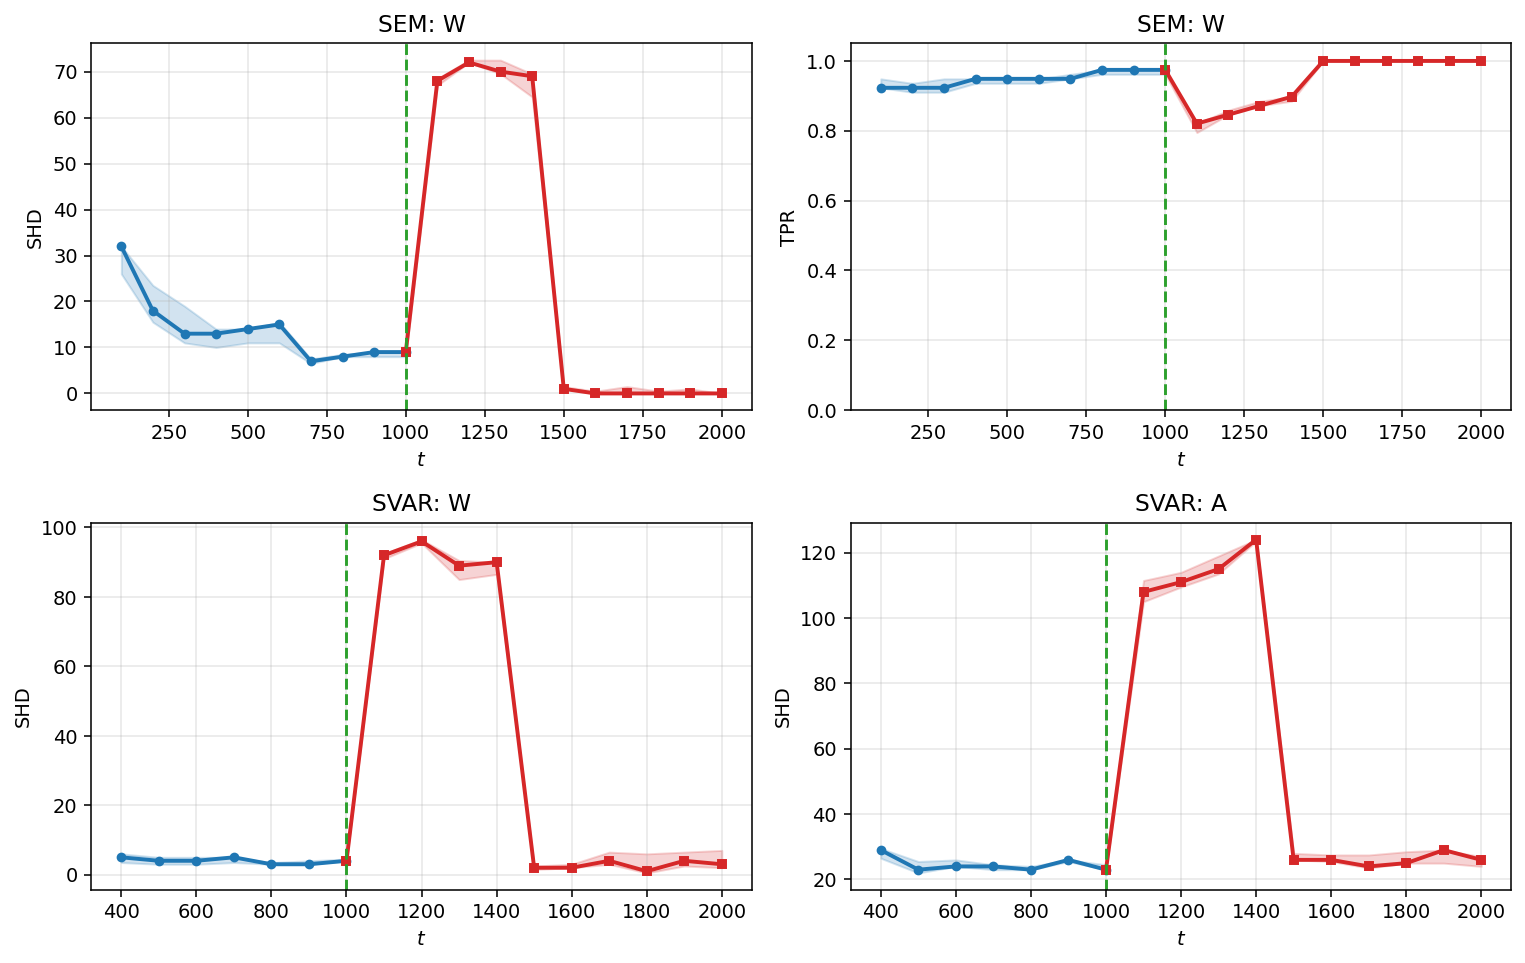
\includegraphics[width=0.74\linewidth]{figures/streaming_evolving_sem_svar.png}
	\end{figure}\svpos

	\bi $d{=}20$, ER2, $\mathrm{batch}{=}100$, window $W{=}500$, change point $t^\star{=}1000$; median over 3 realizations \svpos
	\ai \blue{SEM:} $\bbW$-SHD converges to $9$ pre-change, spikes to $72$ during window mixing, drops to \green{$\mathbf{0}$} (TPR $=1.00$) at $t=1500$
	\ai \blue{SVAR:} $\bbW$-SHD settles at $5\to\mathbf{3}$; $\bbA$-SHD floors $23\to26$ (threshold artifact, not adaptation failure)
	\ai Transition spans exactly $\Theta(W/\mathrm{batch})=5$ batches -- \orange{matching the analysis}\ei

\end{frame}

%%%%%%%%%%%%%%%%%%%%%%%%%%%%%%%%%%%%%%%%%%%%%%%%%%%%%%%%%%%%%%%%
%%%   S   E   C   T   I   O   N   %%%%%%%%%%%%%%%%%%%%%%%%%%%%%%
%%%%%%%%%%%%%%%%%%%%%%%%%%%%%%%%%%%%%%%%%%%%%%%%%%%%%%%%%%%%%%%%
\section{Conclusions}
\begin{frame} \frametitle{Roadmap} \tableofcontents[currentsection] \end{frame}

%%%%%%%%%%%%%%%%%%%%%%%%%%%%%%%%%%%%%%%%%%%%%%%%%%%%%%%%%%%%%%%%
%%%   S   L   I   D   E   %%%%%%%%%%%%%%%%%%%%%%%%%%%%%%%%%%%%%%
%%%%%%%%%%%%%%%%%%%%%%%%%%%%%%%%%%%%%%%%%%%%%%%%%%%%%%%%%%%%%%%%

\begin{frame}{Summary and future work}\svpos

	\bi Proposed an \orange{online DAG learning framework} for streaming data, for both \blue{static (SEM)} and \blue{dynamic (SVAR)} models
	\ai Augments the \green{CoLiDE} family with \darkpurple{running second-order statistics} -- one covariance for SEM, the joint block $(\bbSigma_{XX},\bbSigma_{XY},\bbSigma_{YY})$ for SVAR
	\ai Mini-batch SGD inner loop: \orange{$\ccalO(d^2)$ memory, $\ccalO(d^3)$ time} per step, independent of cumulative samples
	\ai Closed-form noise updates (EV \& NV); Welford backs the true-online $\mathrm{bs}=1$ regime
	\ai \red{Sliding-window} variant tracks evolving DAGs with delay $\Theta(W/\mathrm{batch})$
	\ai \darkred{Streaming $=$ batch} in recovery quality at convergence -- differing only in per-step cost and adaptivity\ei \svpos

	\pause

	\bi \red{\textbf{Ongoing and future work:}}
	\ai \blue{Regret analysis:} $\ccalO(\sqrt{T})$ static and dynamic regret under a path-length budget on $\{\bbW^\star_t\}$
	\ai \blue{Incremental warm-starts:} reuse Adam moments \& schedule index to cut per-batch cost
	\ai \blue{Data-driven thresholds} and online $(\lambda_{\bbW},\lambda_{\bbA})$ schedules
	\ai \blue{Beyond linear/Gaussian:} LiNGAM-style and nonlinear (neural) SEMs; \green{real-data} streaming evaluation\ei

\end{frame}

%%%%%%%%%%%%%%%%%%%%%%%%%%%%%%%%%%%%%%%%%%%%%%%%%%%%%%%%%%%%%%%%

\end{document}
